\chapter{Desarrollo de IPFShare}\label{chap:4desarrollo}
Se ha denominado IPFShare al sistema de intercambio de archivos desarrollado en este proyecto.
\section{Requisitos y definición del sistema}
En esta sección se definen los requisitos funcionales y no funcionales que debe integrar el sistema propuesto.
\subsection{Requisitos funcionales}
\begin{itemize}[noitemsep,after=\vspace{-0.6\baselineskip}]
  \item Un usuario debe poder autenticarse en el sistema.
  \item Un usuario debe poder compartir archivos y directorios con uno o varios usuarios.
  \item Un usuario debe poder descargar archivos y directorios compartidos por otros usuarios del sistema.
  \item A la hora de compartir un archivo un usuario debe poder elegir con qué otros usuarios del sistema compartirlo.
  \item Un usuario debe tener posibilidad de hacer grupos de compartición.
  \item Cuando un usuario comparta recursos con otros usuarios, estos deben recibir una notificación.
  \item Un usuario debe poder interactuar las comparticiones que ha realizado.
  \item Un usuario debe poder interactuar las comparticiones que le han realizado.
\end{itemize}
\subsection{Requisitos no funcionales}
\begin{itemize}[noitemsep,after=\vspace{-0.4\baselineskip}]
  \item El sistema debe proporcionar una interfaz de usuario intuitiva y fácil de usar.
  \item El sistema debe implementar servicios de seguridad en torno a la autenticación.
  \item El sistema debe proporcionar medidas de seguridad para los archivos compartidos.
  \item El sistema debe proporcionar un servicio o mecanismos de identificación de usuario portable.
  \item Las transacciones y eventos del sistema deben ser relativamente instantáneos.
\end{itemize}
Hay que destacar que este sistema no propone la sincronización de archivos que normalmente se asocia con los sistemas de
almacenamiento en la nube. Incluir el desarrollo de esta funcionalidad en el sistema propuesto no es algo trivial.
La sincronización de datos en tiempo real es un tópico muy complejo y se sale
del alcance de este proyecto. Sin embargo, en la sección de \nameref{chap:7trabajosfuturos} dentro de las posibles
mejoras se propone una posible implementación de esta funcionalidad.
\section{Arquitectura y diseño}

Uno de los objetivos de este trabajo es comparar la viabilidad de IPFS como alternativa a los sistemas centralizados.
En esta sección se presenta una arquitectura simplificada para un sistema de intercambio de archivos centralizado habitual.
Después se contrastará con la alternativa descentralizada propuesta.

\subsection{Arquitectura de un sistema de intercambio de archivos centralizado habitual}

Como se puede observar en la figura \ref{fig:centralizedarch}, la arquitectura de un sistema de intercambio de archivos
requiere de varios puntos de acceso centralizados para funcionar\footnote{Este diseño se ha ideado tomando como referencia los siguientes recursos:
  \cite{chakrabortySystemDesignAnalysis2020} y
  \cite{systemdesignSystemDesignInterview2023}.}.En un caso real esta arquitectura podría ser más compleja, pero para este
ejemplo se ha simplificado para centrarse en los puntos clave.

Existe una clara separación conceptual de las distintos componentes, aunque pueden estar ubicados en
el mismo servidor físico, en varios, o incluso, cada servicio en varios servidores físicos. Esto depende de la escala
del sistema y de las necesidades de rendimiento y disponibilidad.

\begin{itemize}[noitemsep,after=\vspace{-0.4\baselineskip}]
  \item \textbf{Almacenamiento cloud:} el almacén donde se guardarán los chunks de ficheros proporcionados por el servicio
        de procesamiento de ficheros, Amazon S3 es un ejemplo de un servicio de estas característica.
        \item\textbf{Servicio de procesamiento de ficheros:} es el encargado atender y llevar a cabo las peticiones de usuario relacionadas con ficheros.
  \item \textbf{Servicio de autenticación:} gestiona la autenticación de los usuarios. Contiene los datos de los usuarios y sus credenciales.
  \item \textbf{Servicio de metadatos:} se encarga de enviar las notificaciones de los usuarios. Cuando un cliente
        comparte un fichero con otro, el cliente envía también una serie de metadatos sobre esta acción que acaba de realizar.
        Estos metadatos se pueden usar para gran variedad de propósitos. En este caso se usan para implementar un servicio de notificaciones basado en colas de mensajes.
\end{itemize}
\afterpage{
  \begin{sidewaysfigure}
    \centering
    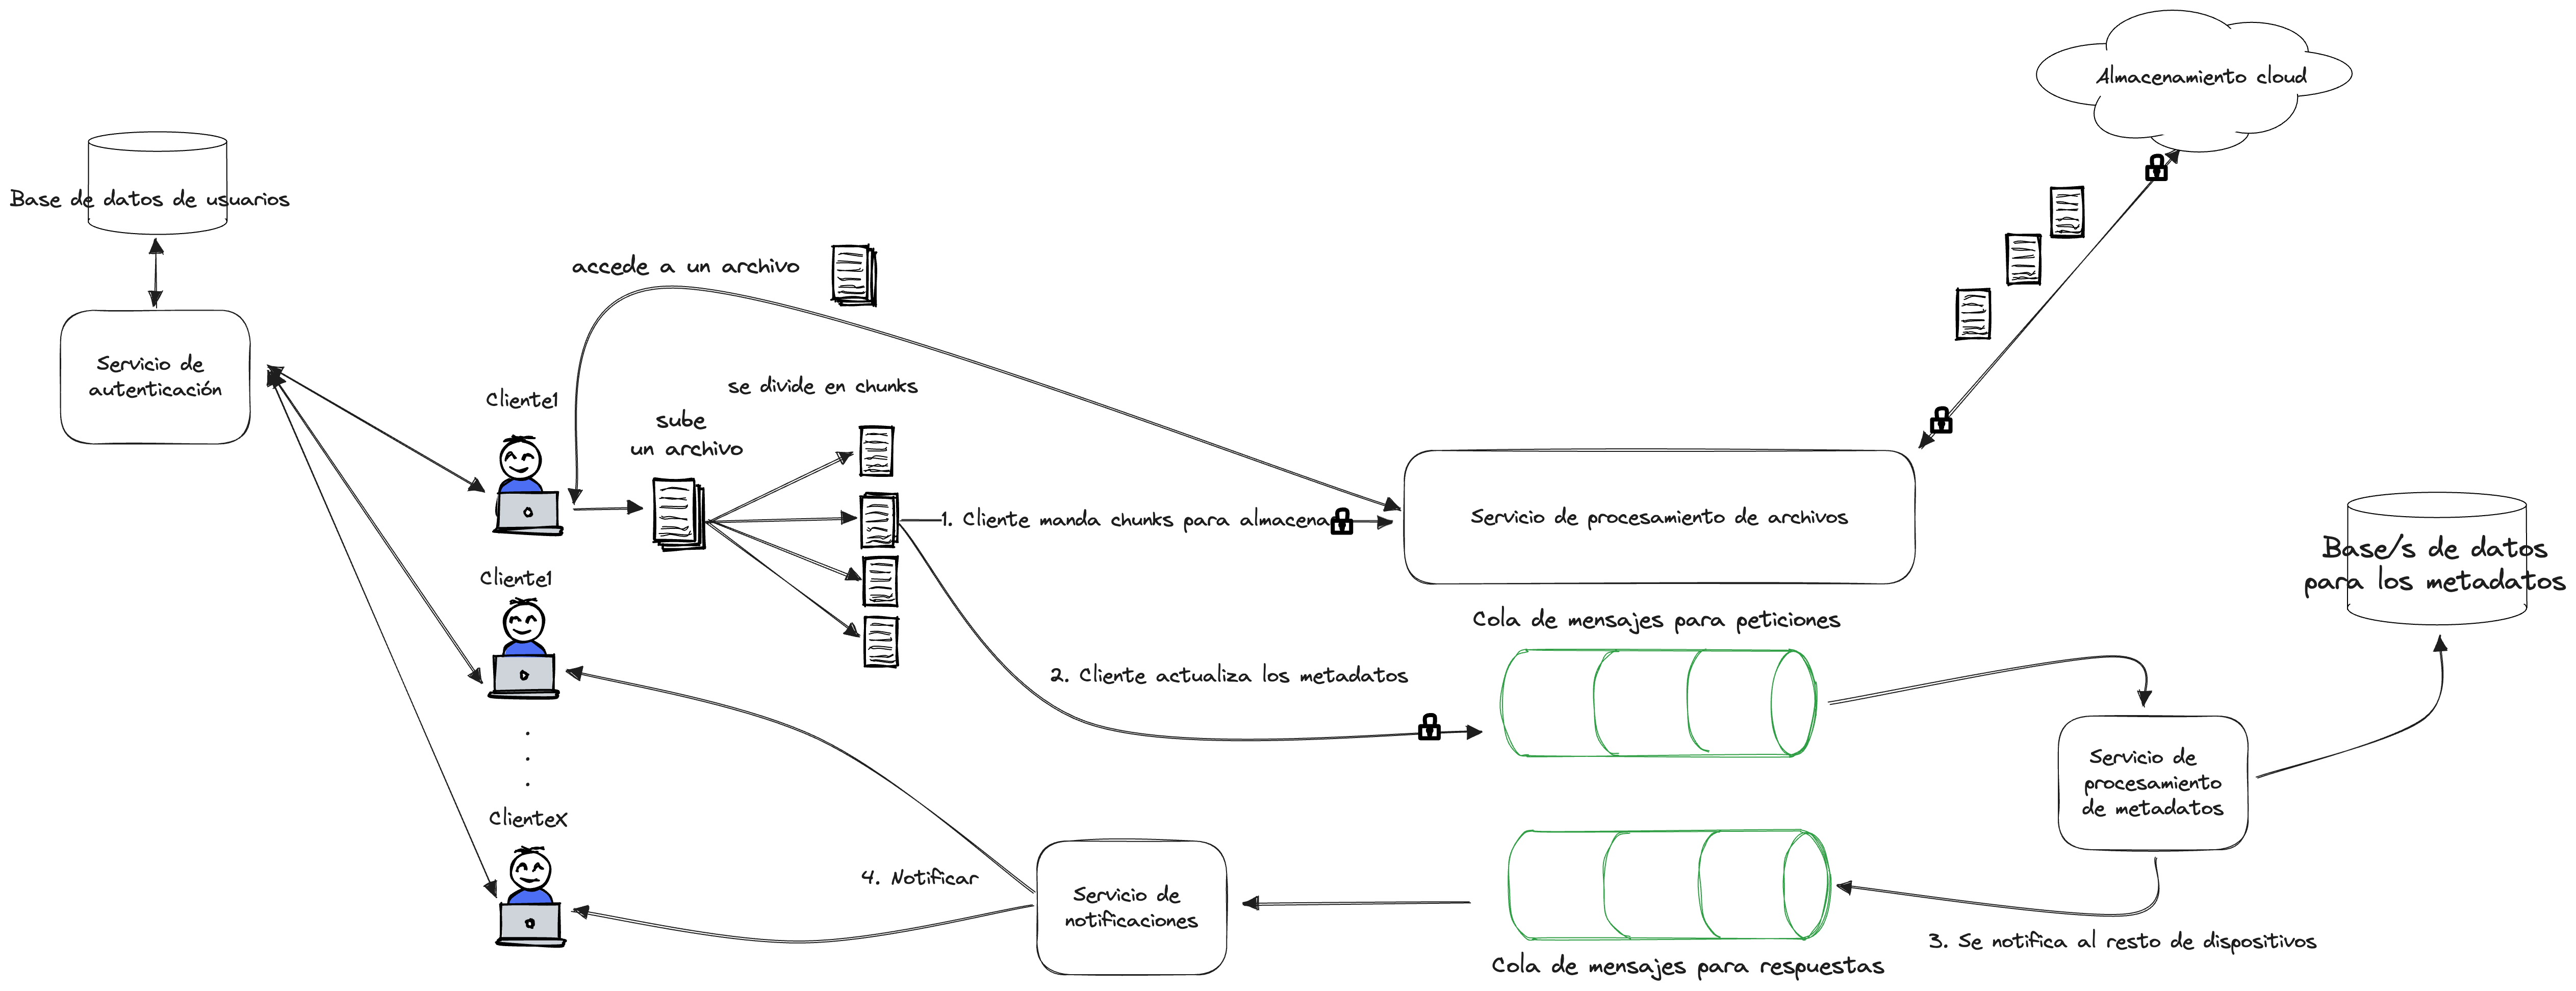
\includegraphics[width=\textwidth]{images/diagramacentral.png}
    \caption{Posible arquitectura de un servicio centralizado de archivos}
    \label{fig:centralizedarch}
  \end{sidewaysfigure}
}

Cuando un cliente quiere compartir un fichero, este divide el archivo en trozos más pequeños llamados chunks\footnote{En un servicio de compartición de archivos, los archivos se subdividen en fragmentos o chunks para mejorar la eficiencia de la transferencia de datos, permitiendo la transmisión paralela y la reanudación de las transferencias interrumpidas, así como facilitar la distribución del almacenamiento y reducir la redundancia de datos.}.
Envía a través de una conexión segura (socket tpc sobre TLS por ejemplo) estos chunks que componen el archivo al servicio de procesamiento de ficheros.
Este servicio se encarga de guardar los chunks en el almacenamiento cloud y de mandar los metadatos a la cola de mensajes.
El servicio de metadatos procesa de forma asíncrona estos metadatos, extrayendo la información pertinente que identifique
a los usuarios y el recurso compartido. Después envía una notificación a los usuarios que corresponda.

Dado que el servicio de autenticación posee datos de los usuarios, cuando un usuario quiera enviar un archivo puede
pedir esta al servicio de autenticación, el incluso se podría combinar con el servicio de metadatos para brindar otras funcionalidades como ver los recursos que se le han compartido o los usuarios con los que se ha compartido.

Bajo este sistema los clientes deben saber de antemano dónde se ubican estos servicios para poder interactuar con
ellos. Estos servicios podrían ser provistos por entidades externas, por lo que el sistema no sería completamente autocontenido, existiendo dependencias en sistemas centralizados de terceros.

\subsection{Arquitectura de IPFShare: un sistema de intercambio de archivos descentralizado}
En comparacion con la arquitectura anterior (figura \ref{fig:centralizedarch}), la arquitectura de IPFShare (figura \ref{fig:ipfssharearch}) es completamente descentralizada.
\section{Tecnologías}
\subsection{Tecnologías propuestas}
\subsection{Tecnologías usadas}


\section{Implementación}


\begin{minted}{typescript}
import OrbitDB from "orbit-db"
// eslint-disable-next-line @typescript-eslint/ban-ts-comment
// @ts-ignore
import AccessController from "orbit-db-access-controllers/interface"
import DocumentStore from "orbit-db-docstore"
import { IdentityProvider } from "orbit-db-identity-provider"

export interface RegistryEntry {
    peerId: string
    orbitdbIdentity: string // DID
    username: string // alias
  }

export abstract class Registry<S, DocType> {
    abstract accessController: AccessController
    abstract store: S
    abstract open(): Promise<void>
    abstract create(): Promise<void>
    abstract replicate(): Promise<void>
    abstract close(): Promise<void>
    abstract addUser(user: DocType): Promise<void>
    abstract getUser(entryId: string): Promise<DocType | undefined>
    abstract updateUser(entryId: string, updates: Partial<DocType>): Promise<void>
    abstract searchUsers(queryFn: (entry: DocType) => boolean): Promise<DocType[]>
    abstract deleteUser(entryId: string): Promise<void>
  }
\end{minted}